\begin{nestedsection}{R4 System: Rule-based Reasoning over RDF streams using Rete}{implementation}
	As a proof of concept for the CoDeR model, we have implemented R4: a Rule-based Reasoner for RDF-streams using Rete.
	Reasoning in R4 is performed continuously and incrementally as dataflow networks that work directly on RDF streams, constructed according to the Rete pattern matching algorithm \citep{forgy79}.
	The system architecture is shown in \reffig{R4-architecture}.
	\begin{figure}[b]
		\centering
		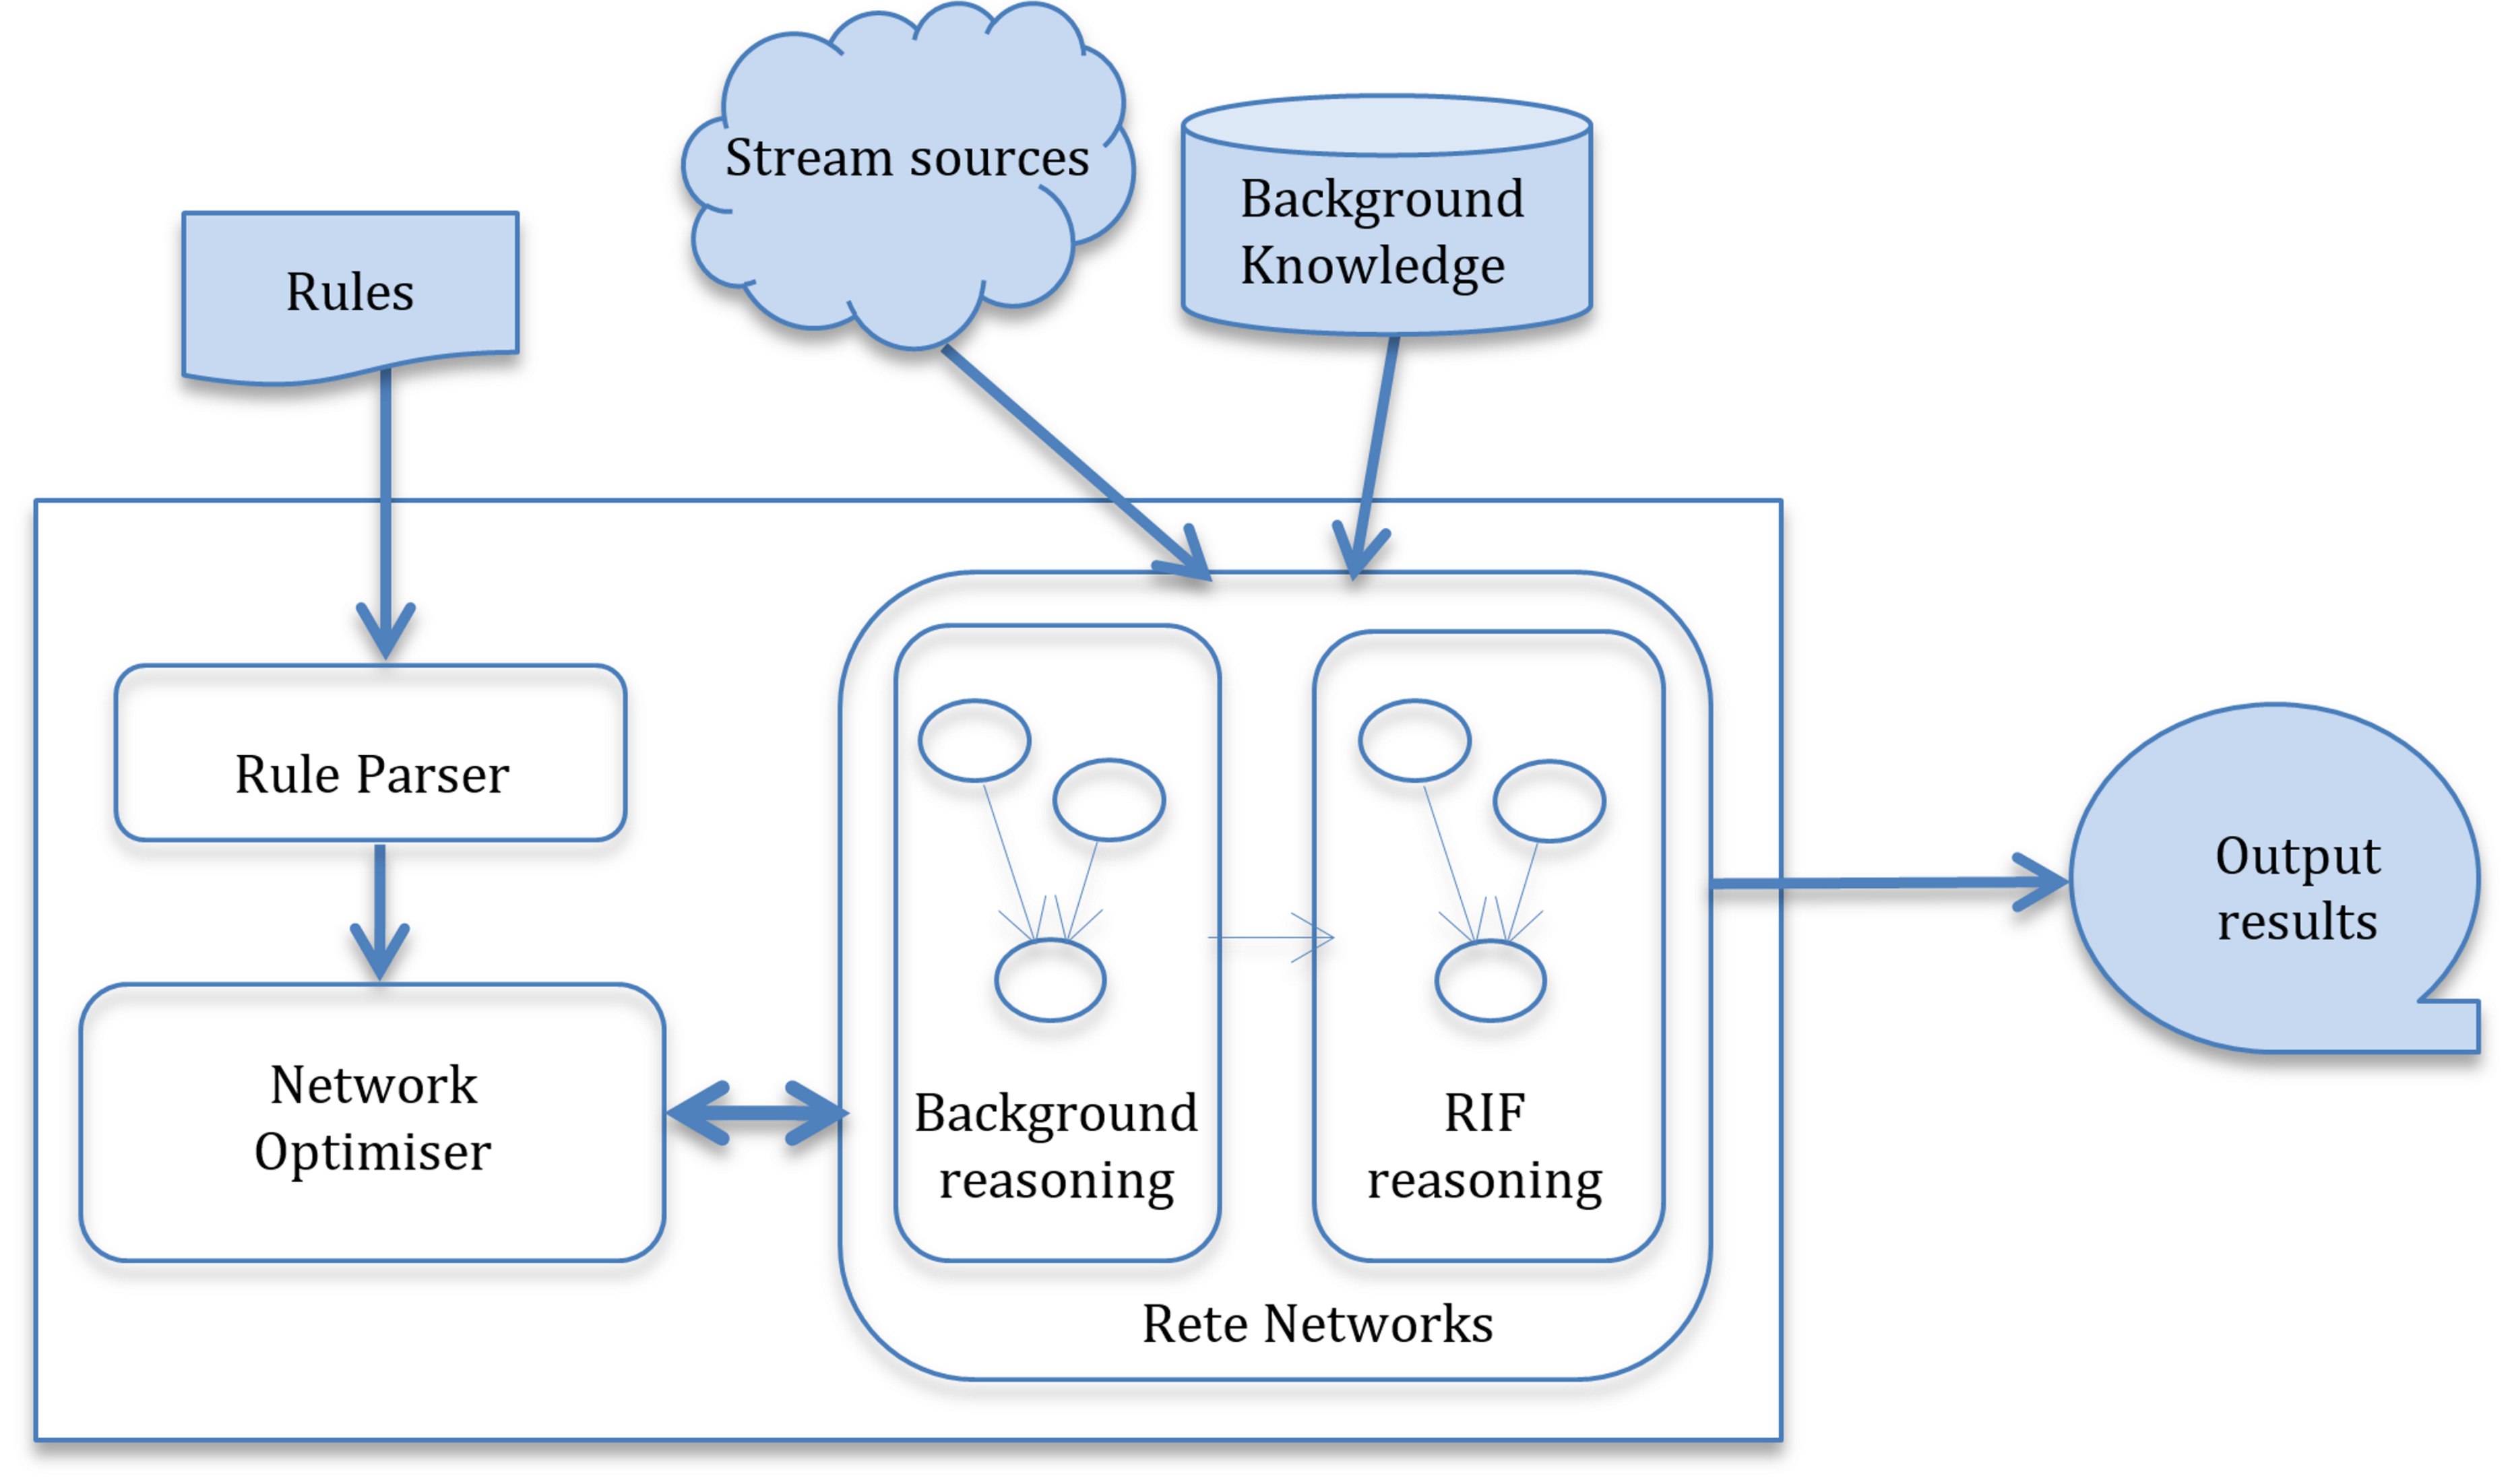
\includegraphics[width=0.45\textwidth]{R4-architecture.png}
		\caption{The system architecture of R4.}
		\labelfig{R4-architecture}
	\end{figure}

	\begin{figure*}[t]
		\centering
		\begin{ebnf}
			\Rule{Document}{
			        \Optional{\NTerm{IRIMETA}} 
			        \Token{Document} 
			        \Token{(} 
			        \Optional{\NTerm{Base}} 
			        \ZeroOrMore{\NTerm{Prefix}} 
			        \ZeroOrMore{\NTerm{Import}}
			        \Optional{\NTerm{Window}}
			        \Optional{\NTerm{Group}} 
			        \Token{)}
			}
			\Rule{Base}{
			        \Token{Base} 
			        \Token{(} 
			        \NTerm{ANGLEBRACKIRI} 
			        \Token{)}
			}
			\Rule{Prefix}{
			        \Token{Prefix} 
			        \Token{(} 
			        \NTerm{Name} 
			        \NTerm{ANGLEBRACKIRI} \Token{)}
			}
			\Rule{Import}{
			        \Optional{\NTerm{IRIMETA}} 
			        \Token{Import} 
			        \Token{(} 
			        \NTerm{LOCATOR} 
			        \Optional{\NTerm{PROFILE}} 
			        \Token{)}
			}
			\Rule{Group}{
			        \Optional{\NTerm{IRIMETA}} 
			        \Token{Group} 
			        \Token{(} 
			        \ZeroOrMore{\OrList{\NTerm{RULE} \OrSep \NTerm{Group}}} 
			        \Token{)}
			}
			\Rule{RULE}{
			        \Optional{\NTerm{IRIMETA}}
			        \Token{Forall}
			        \OneOrMore{\NTerm{Variable}}
			        \Token{(}
			        \NTerm{CLAUSE}
			        \Token{)}
			}
			\OrRule{
			        \NTerm{CLAUSE}
			}
			\Rule{CLAUSE}{
			        \OrList{\NTerm{Implies} \OrSep \NTerm{ATOMIC}}
			}
			\Rule{Implies}{
			        \Optional{\NTerm{IRIMETA}}
			        \OrList{\NTerm{ATOMIC} \OrSep \Token{And} \Token{(} \ZeroOrMore{ATOMIC} \Token{)}}
			        \Token{:-}
			        \NTerm{FORMULA}
			}
			\Rule{LOCATOR}{
			        \NTerm{ANGLEBRACKURI}
			}
			\Rule{PROFILE}{
			        \NTerm{ANGLEBRACKURI} 
			}
			\Rule{Window}{
			        \NTerm{Number}
			        \NTerm{TimeUnit}
			}
			\Rule{TimeUnit}{
			        \OrList{\Token{ms} \OrSep \Token{s} \OrSep \Token{m} \OrSep \Token{h}}
			}
		\end{ebnf}
		\caption{Streaming RIF-Core Grammar}
		\labelfig{lst-S-RIF-Core}
	\end{figure*}

	A rule document containing any number of rules is submitted to the system.
	We have chosen RIF-Core to be the language in which rules can be represented, for being compatible with RDF and other semantic web standards, as well as sharing the semantics of positive Datalog.
	The rule document specifies any domain-specific rules as well as an entailment regime \emph{if any} for background reasoning.
	We also added a simple extension to RIF-Core in line with the extension of Datalog described in \refsec{semantics}, enabling users to specify a window range as part of their rule set, as shown in \reffig{lst-S-RIF-Core}.
	Further, we propose the extension of the set of `PROFILE's that describe the `Import's of a rule set to include those definitions of RDF streams recognised by the W3C.

	These rules are translated by the rule parser into a set of objects that are then used by the network optimizer to generate the Rete-like dataflow networks.
	The optimizer employs simple known heuristics to generate a good plan.
	These heuristics include: sharing nodes between rules where the sub-graph patterns their results match are variants of each other; avoiding Cartesian products as much as possible by joining patterns that have common variables earlier in the beta network; and pushing more selective patterns (those with fewer variables) earlier in the alpha network to minimize intermediate results.
	
	The optimizer instantiates a Rete network for background reasoning if required and another network for generic rules.
	The first network feeds into the second one and the two together are ``re-entrant'', meaning that the first network takes as input the stream of entailments produced by both the first and the second, to enable iterative inference of results such as the calculation of transitive closure.
	
	These networks receive streaming data in the form of sequences of RDF graphs, and operate directly on each of these graphs incrementally.
	We chose this RDF-native approach as opposed to reusing existing technologies as in \citep{C-SPARQL,streaming-sparql} to allow full control over the low-level operators.
	This can offer maximum optimization opportunities such as adaptively optimizing the network topologies, which is part of our future work.

	\begin{nestedsection}{Continuous Reasoning with Rete}{implementation: continuous rete}
		The Rete algorithm \citep{forgy79}, which was introduced as a solution for the many pattern/many object matching problem, can be well fit into the stream reasoning model as it operates incrementally.
		The RETE algorithm can process large data sets efficiently because it avoids iterating over both data elements (facts, or ``working memory'') and over the production rules.
		To avoid iteration over data elements, the RETE algorithm stores with each condition (or pattern), a list of the data elements that it matches.
		These lists are updated when the working memory changes, in a forward chaining process.
		To avoid iteration over the production rules, the RETE algorithm creates a dataflow tree-structured network to represent the rules.

		However, the Rete algorithm is memory-intensive as it stores all partial matches, trading memory for speed.
		In a streaming context, this is infeasible as streams can grow without bounds.
		Therefore, we place time constraints on the memories using a window-join operator instead of the traditional incremental joins.
	\end{nestedsection}
	\begin{nestedsection}{Continuous Reasoning in the Semantic Web}{implementation: continuous reasoning with RDF}
		\begin{figure*}[t]
 			\centering
 			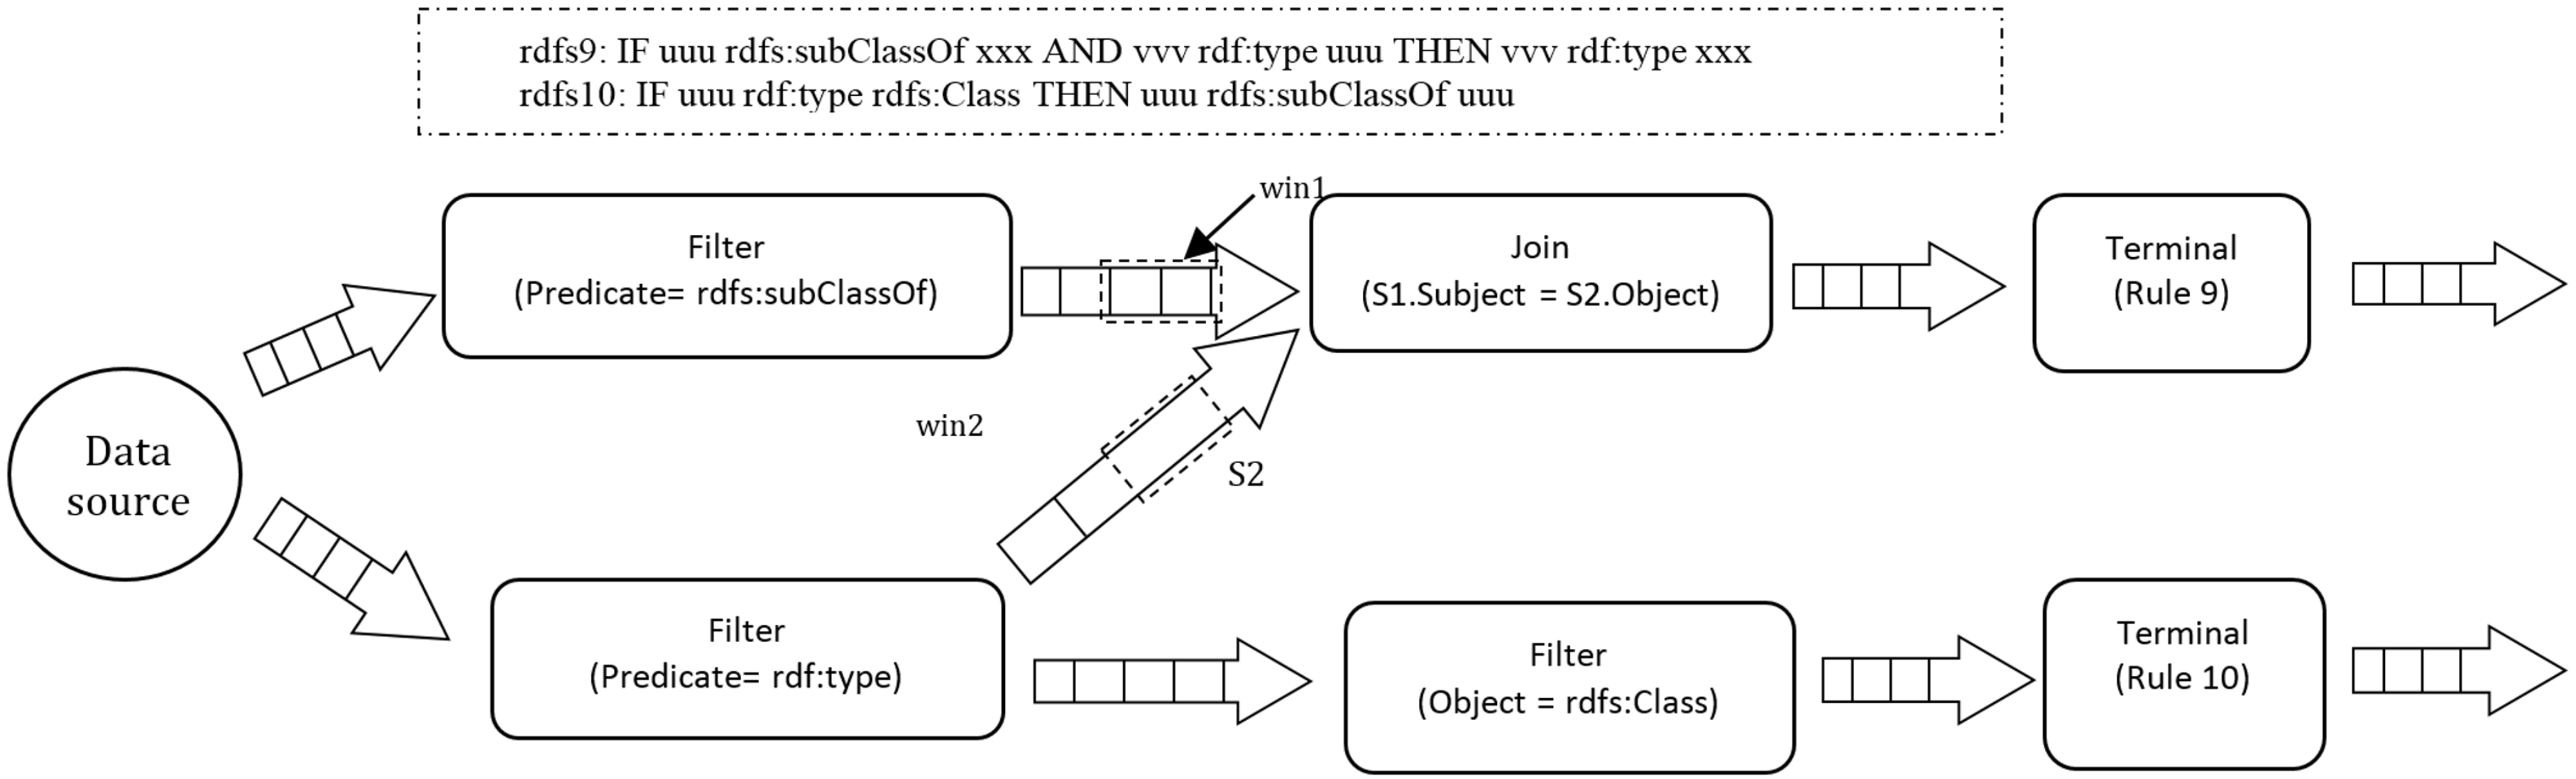
\includegraphics[width=0.9\textwidth]{example-rete-network.png}
 			\caption{An example Rete network with corresponding (RDFS) rules.}
 			\labelfig{example-rete-network}
 		\end{figure*}
		In R4, data enters the network through the source nodes, which convert streams of graphs into streams of quads, by extracting the graph ID and attaching it to every triple in this graph.
		Source nodes are, therefore, implementations of the graph-to-stream operator ${{}_g{\pi_t}}$ of CoDeR.
		Source nodes also annotate the incoming quads with the system time at their arrival if their parent graph was not already annotated at its origin, otherwise passing the annotation of the graph to the resulting quads.
		This annotation $a$ relates to their instant of assertion $e$ within the CoDeR data model, and the instant $n$ at which they will leave the window whose range $r$ is defined in the system's rule set may be derived by ${n = a + r}$.
		Source nodes propagate the annotated quads to their successor nodes, which are the alpha nodes.

		Alpha nodes are single-entry nodes that form a discrimination network, as shown in \reffig{example-rete-network}.
		In R4, alpha nodes can receive streamed quads from any number of nodes through its single input, reflecting the multiple-source nature of CoDeR's streams.
		Each received quad is matched against some conditions, and is either dropped if there is no match, or propagated downstream to its successor node(s) in the case of a match.
		As such, R4's interpretation of alpha nodes are implementations of the triple-select operator $\sigma_{triple}$ of CoDeR, but can also filter based on the datatypes of the values in triples, thereby also implementing the other selection operator of CoDeR, $\sigma_{external}$.

		The first alpha node in the network propagates matched quads to a special node called the left input adaptor, while the other alpha nodes propagate their output directly to beta nodes.
		The left input adaptor node is responsible of preparing the incoming quads to enter the beta network from the left input of the first beta node in a given join-tree.
		It creates a new \emph{token} that represents a partial match, defined as a list of quads, for each rule body for which the incoming quad is a sub-graph match, then adds this quad as the first item in each list.
		It also annotates each token with the same time as was the quad for which it was generated.
		Tokens are then sent to the first nodes in the beta network.

		Beta nodes are two-input nodes that are responsible for joining the branches of the alpha network, as demonstrated in \reffig{example-rete-network}.
		In our implementation, as in the original Rete algorithm, beta nodes form a left-deep tree.
		Each beta node maintains a left memory, which is a beta memory storing tokens received from other beta nodes (or from the left input adaptor node in case of the first beta node) and a right memory, which is an alpha memory storing quads received from alpha nodes.
		Join nodes are beta nodes that match graphs from both sides according to some conditions, e.g. a shared variable binding.
		As explained earlier, we use stream-to-stream window-join operators to avoid storing and operating over all partial results.
		In this context, each left (beta) and right (alpha) memory is implemented as a \emph{valid window}.
		These windows are implemented as priorities queues in which quads are ordered according to their time annotations, and pruned by ``popping'' from the queue and deleting any quads whose annotation $a \leqslant i - r$, where $i$ is the current system time and $r$ is the range of the semantic window.

		When a join node is left activated, i.e. it receives a token through its left input, it first adds the new token to its left window, then it prunes its right window before iterating over the remaining quads to find any matches.
		When a match is found, a new token is created by duplicating the left token and adding the right quad to the new token's quad list.
		The new token is annotated with the \emph{earliest} time with which its component quads were annotated, and then propagated to the next beta node, or to the terminal node if it is in the root node of a join tree.
		Conversely, when the join node is right activated by receiving a quad from an alpha node, it adds the new quad to the right window, prunes the left window then matches the quad against the remaining tokens.

		This method of annotating tokens with the earliest assertion time of those of its components initially appears to violate the annotation semantics for entailed fact instances laid out in \refsec{semantics,model}.
		However, the ordering of tokens in their streams and the system time $i$ at which they are propagated through the system expresses implicitly CoDeR's entailment time $e$ of entailed instances.
		This leaves the annotation $a$ of a token in R4, in combination with the range $r$ of the semantic window associated with the rule set, able to express CoDeR's negation time ${n}$ of entailed instances by the same calculation as those of asserted instances: ${n = a + r}$.
		As such, the interpretation of beta nodes in R4 is a valid implementation of the window-join operator characterised as a pair of CoDeR SteMs $\rstreamjoin$ implicitly unioned by contribution to the same stream, as shown in \reffig{continuous datalog: SteM}.

		Finally, terminal nodes receive tokens from the root nodes of join-trees and are responsible for producing entailed graphs, directly implementing the instance entailment operator $\text{:-}_{head}$ of CoDeR.
		As with the $\text{:-}_{head}$ operator, the annotation of these entailed graphs is directly inherited from the completed token from which it is produced.
 		The union of the output of all terminal nodes is both the output of the system itself, and re-entered as an input stream to the source nodes to support iterative inference.
	\end{nestedsection}
\end{nestedsection}
